\subsection{Fonctionnement interne de Simterpose}
\label{subsection:fonctionnement_simterpose}

Les actions à intercepter pour maintenir la virtualisation sont de différentes
natures. Il peut s'agir d'actions liées aux communications réseaux, à la
création et à l'identification des processus, à la gestion du temps, ainsi qu'à
l'utilisation du protocole DNS. Pour chacune, les outils utilisés ne sont pas
nécessairement les mêmes. Nous allons donc voir lesquels sont employés parmi
ceux cités dans la section \ref{section:tools}.

\subsubsection{Les communications réseaux}
 %-> syscall -> ptrace (full mediation, address translation)
\label{subsubsection:fonctionnement_reseau}

Dans le cas d'une communication réseau, le but de Simterpose étant de réussir à
simuler un réseau virtuel sur un réseau local, il faut gérer la transition entre
réseau local et réseau simulé, comme le montre la Figure \ref{COMM}. En effet,
l'application possède une adresse IP et des numéros de ports virtuels qui ne
correspondent pas à ceux attribués dans le réseau local.

La gestion de cette transition va se faire au niveau des appels systèmes, car nous ne souhaitons pas oublier des fonctions en utilisant \texttt{LD\_PRELOAD}. Pour intercepter les appels systèmes liés au réseau nous allons utiliser l'appel système \texttt{ptrace} présenté en section \ref{subsection:ptrace}.

\begin{figure}[H]
  \centering
  \begin{subfigure}{0.5\textwidth}
    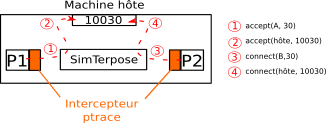
\includegraphics[scale=0.8]{Pictures/png/Mediation_realite}
    \caption{Communications réelles}
  \label{COMM_REALITE}
  \end{subfigure}
  \begin{subfigure}{0.25\textwidth}
  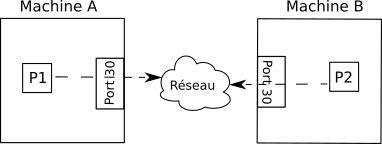
\includegraphics[scale=0.5]{Pictures/png/Mediation_VM}
  \caption{Communications vues \\ par les processus}
  \label{COMM_VM}
  \end{subfigure}
  \caption{Les communications réseau entre deux processus}
  \label{COMM}
\end{figure}

De plus, il n'est pas suffisant de se baser uniquement sur le descripteur de fichier associé à une socket pour identifier deux entités qui communiquent
entre elles. En effet ce descripteur est unique pour chaque socket
d'un processus, mais plusieurs processus peuvent avoir un même descripteur de fichier pour des sockets de communications différentes puisque
chacun à son propre espace mémoire. Pour pallier à ce problème, nous allons utiliser les adresses IP et les ports locaux et distants des
deux entités qui souhaitent communiquer comme moyen d'identification en plus du numéro de socket.

Afin de gérer toutes ces modifications deux solutions ont été proposées lors
d'un précédent stage \citep{GUILLAUME:Interceptionsyscall}: l'\textit{address
  translation} et la \textit{full mediation}. Néanmoins, ces deux solutions
n'ont pas encore été évaluée en pratique.
 
\paragraph{Traduction d'adresse}
 Avec ce type de médiation, illustrée Figure \ref{ADDRESS_TRANSLATION}, on laisse le noyau gèrer les communications. Ainsi, en entrée et sortie d'appel système, Simterpose va juste s'occuper de la transition entre le réseau virtuel simulé
 par SimGrid et le réseau local, en utilisant les informations de communications
 contenues dans la socket. Pour cela, Simterpose gère un tableau de
 correspondances, dans lequel pour chaque couple <IP, ports>virtuels , on a un
 couple <IP, ports>réels associé.  De fait, en entrée d'un appel système de
 type réseau (\texttt{bind}, \texttt{connect}, \texttt{accept} ...), Simterpose
 doit remplacer l'adresse et les ports virtuels de l'application par l'adresse
 et les ports réels sur le réseau local, afin que la source de l'appel système
 corresponde à une machine existante sur le réseau local. Au retour de l'appel
 système, il faudra remodifier les paramètres en remettant l'adresse et les
 ports virtuels. La limite de cette approche est liée au nombre de
 ports disponibles sur l'hôte.

\paragraph{Full mediation} \label{paragraph:FULL_MEDIATION}
Dans ce cas, le noyau ne va plus gérer les communications car nous allons
empêcher l'application de communiquer via des sockets et même d'établir des
connexions avec une autre application. Puisqu'il n'y a aucune communication, on
n'a pas besoin de gérer de tableau de correspondance d'adresses et de ports et
les applications peuvent conserver les adresses et les ports simulés qu'elles
considèrent comme réels. Quand l'application voudra faire un appel système de
type communication ou connexion vers une autre application, le processus espion
de Simterpose qui sera notifié via \texttt{ptrace} neutralisera l'appel système,
comme illustré sur la Figure \ref{FULL_MEDIATION}. Ensuite, ce processus
récupérera, en lisant dans la mémoire du processus espionné, les données à
envoyer ou récupérer et ira directement les lire ou les écrire dans la mémoire
du destinataire.

\begin{figure}[H]
   \centering
   \begin{subfigure}{0.5\textwidth}
   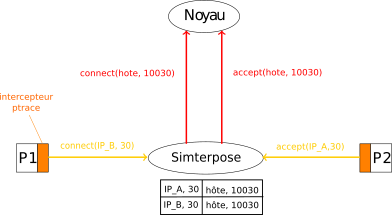
\includegraphics[scale=0.5]{Pictures/png/Mediation_translation_v2}
   \caption{\textit{Address translation}}
   \label{ADDRESS_TRANSLATION}
   \end{subfigure}
   \begin{subfigure}{0.4\textwidth}
     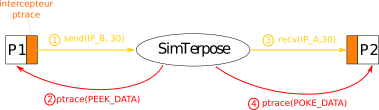
\includegraphics[scale=0.5]{Pictures/png/Mediation_full_v2}
  \caption{\textit{Full mediation}}
  \label{FULL_MEDIATION}
   \end{subfigure}
   \caption{Les différents types de médiation}
   \label{MEDIATION}
 \end{figure}
